\ifdefined\included
\else
\documentclass[english,a4paper,11pt,twoside]{StyleThese}
\usepackage{amsmath,amssymb}             % AMS Math
\usepackage[T1]{fontenc}
\usepackage[utf8x]{inputenc}
\usepackage{babel}
\usepackage{datetime}

\usepackage{lmodern}
\usepackage{tabularx}
%\usepackage{tabular}
\usepackage{multirow}

\usepackage{subfigure}
\usepackage{fancyvrb}
\usepackage{algorithmic}
\usepackage{algorithm}
\usepackage{mathtools}


\usepackage{hhline}
\usepackage[left=1.5in,right=1.3in,top=1.1in,bottom=1.1in,includefoot,includehead,headheight=13.6pt]{geometry}
\renewcommand{\baselinestretch}{1.05}

% Table of contents for each chapter

\usepackage[nottoc, notlof, notlot]{tocbibind}
\usepackage{minitoc}
\setcounter{minitocdepth}{2}
\mtcindent=15pt
% Use \minitoc where to put a table of contents

\usepackage{aecompl}


% Glossary / list of abbreviations

\usepackage[intoc]{nomencl}
\iftoggle{ThesisInEnglish}{%
\renewcommand{\nomname}{Glossary}
}{ %
\renewcommand{\nomname}{Liste des Abréviations}
}

\newcommand{\accom}[1]{\textcolor{red}{[#1]}}

\makenomenclature

% My pdf code

\usepackage{ifpdf}

\ifpdf
  \usepackage[pdftex]{graphicx}
  \DeclareGraphicsExtensions{.jpg}
  \usepackage[a4paper,pagebackref,hyperindex=true]{hyperref}
  \usepackage{tikz}
  \usetikzlibrary{arrows,shapes,calc}
\else
  \usepackage{graphicx}
  \DeclareGraphicsExtensions{.ps,.eps}
  \usepackage[a4paper,dvipdfm,pagebackref,hyperindex=true]{hyperref}
\fi

\graphicspath{{.}{images/}}

%% nicer backref links. NOTE: The flag ThesisInEnglish is used to define the
% language in the back references. Read more about it in These.tex

\iftoggle{ThesisInEnglish}{%
\renewcommand*{\backref}[1]{}
\renewcommand*{\backrefalt}[4]{%
\ifcase #1 %
(Not cited.)%
\or
(Cited in page~#2.)%
\else
(Cited in pages~#2.)%
\fi}
\renewcommand*{\backrefsep}{, }
\renewcommand*{\backreftwosep}{ and~}
\renewcommand*{\backreflastsep}{ and~}
}{%
\renewcommand*{\backref}[1]{}
\renewcommand*{\backrefalt}[4]{%
\ifcase #1 %
(Non cité.)%
\or
(Cité en page~#2.)%
\else
(Cité en pages~#2.)%
\fi}
\renewcommand*{\backrefsep}{, }
\renewcommand*{\backreftwosep}{ et~}
\renewcommand*{\backreflastsep}{ et~}
}

% Links in pdf
\usepackage{color}
\definecolor{linkcol}{rgb}{0,0,0.4} 
\definecolor{citecol}{rgb}{0.5,0,0} 
\definecolor{linkcol}{rgb}{0,0,0} 
\definecolor{citecol}{rgb}{0,0,0}
% Change this to change the informations included in the pdf file

\hypersetup
{
bookmarksopen=true,
pdftitle="Joint Action for Human-Robot Interaction",
pdfauthor="Sandra DEVIN", %auteur du document
pdfsubject="Thesis", %sujet du document
%pdftoolbar=false, %barre d'outils non visible
pdfmenubar=true, %barre de menu visible
pdfhighlight=/O, %effet d'un clic sur un lien hypertexte
colorlinks=true, %couleurs sur les liens hypertextes
pdfpagemode=None, %aucun mode de page
pdfpagelayout=SinglePage, %ouverture en simple page
pdffitwindow=true, %pages ouvertes entierement dans toute la fenetre
linkcolor=linkcol, %couleur des liens hypertextes internes
citecolor=citecol, %couleur des liens pour les citations
urlcolor=linkcol %couleur des liens pour les url
}

% definitions.
% -------------------

\setcounter{secnumdepth}{3}
\setcounter{tocdepth}{2}

% Some useful commands and shortcut for maths:  partial derivative and stuff

\newcommand{\pd}[2]{\frac{\partial #1}{\partial #2}}
\def\abs{\operatorname{abs}}
\def\argmax{\operatornamewithlimits{arg\,max}}
\def\argmin{\operatornamewithlimits{arg\,min}}
\def\diag{\operatorname{Diag}}
\newcommand{\eqRef}[1]{(\ref{#1})}

\usepackage{rotating}                    % Sideways of figures & tables
%\usepackage{bibunits}
%\usepackage[sectionbib]{chapterbib}          % Cross-reference package (Natural BiB)
%\usepackage{natbib}                  % Put References at the end of each chapter
                                         % Do not put 'sectionbib' option here.
                                         % Sectionbib option in 'natbib' will do.
\usepackage{fancyhdr}                    % Fancy Header and Footer

% \usepackage{txfonts}                     % Public Times New Roman text & math font
  
%%% Fancy Header %%%%%%%%%%%%%%%%%%%%%%%%%%%%%%%%%%%%%%%%%%%%%%%%%%%%%%%%%%%%%%%%%%
% Fancy Header Style Options

\pagestyle{fancy}                       % Sets fancy header and footer
\fancyfoot{}                            % Delete current footer settings

%\renewcommand{\chaptermark}[1]{         % Lower Case Chapter marker style
%  \markboth{\chaptername\ \thechapter.\ #1}}{}} %

%\renewcommand{\sectionmark}[1]{         % Lower case Section marker style
%  \markright{\thesection.\ #1}}         %

\fancyhead[LE,RO]{\bfseries\thepage}    % Page number (boldface) in left on even
% pages and right on odd pages
\fancyhead[RE]{\bfseries\nouppercase{\leftmark}}      % Chapter in the right on even pages
\fancyhead[LO]{\bfseries\nouppercase{\rightmark}}     % Section in the left on odd pages

\let\headruleORIG\headrule
\renewcommand{\headrule}{\color{black} \headruleORIG}
\renewcommand{\headrulewidth}{1.0pt}
\usepackage{colortbl}
\arrayrulecolor{black}

\fancypagestyle{plain}{
  \fancyhead{}
  \fancyfoot{}
  \renewcommand{\headrulewidth}{0pt}
}

%\usepackage{MyAlgorithm}
%\usepackage[noend]{MyAlgorithmic}
\usepackage[ED=MITT - STICIA, Ets=INP]{tlsflyleaf}
%%% Clear Header %%%%%%%%%%%%%%%%%%%%%%%%%%%%%%%%%%%%%%%%%%%%%%%%%%%%%%%%%%%%%%%%%%
% Clear Header Style on the Last Empty Odd pages
\makeatletter

\def\cleardoublepage{\clearpage\if@twoside \ifodd\c@page\else%
  \hbox{}%
  \thispagestyle{empty}%              % Empty header styles
  \newpage%
  \if@twocolumn\hbox{}\newpage\fi\fi\fi}

\makeatother
 
%%%%%%%%%%%%%%%%%%%%%%%%%%%%%%%%%%%%%%%%%%%%%%%%%%%%%%%%%%%%%%%%%%%%%%%%%%%%%%% 
% Prints your review date and 'Draft Version' (From Josullvn, CS, CMU)
\newcommand{\reviewtimetoday}[2]{\special{!userdict begin
    /bop-hook{gsave 20 710 translate 45 rotate 0.8 setgray
      /Times-Roman findfont 12 scalefont setfont 0 0   moveto (#1) show
      0 -12 moveto (#2) show grestore}def end}}
% You can turn on or off this option.
% \reviewtimetoday{\today}{Draft Version}
%%%%%%%%%%%%%%%%%%%%%%%%%%%%%%%%%%%%%%%%%%%%%%%%%%%%%%%%%%%%%%%%%%%%%%%%%%%%%%% 

\newenvironment{maxime}[1]
{
\vspace*{0cm}
\hfill
\begin{minipage}{0.5\textwidth}%
%\rule[0.5ex]{\textwidth}{0.1mm}\\%
\hrulefill $\:$ {\bf #1}\\
%\vspace*{-0.25cm}
\it 
}%
{%

\hrulefill
\vspace*{0.5cm}%
\end{minipage}
}

\let\minitocORIG\minitoc
\renewcommand{\minitoc}{\minitocORIG \vspace{1.5em}}

\usepackage{multirow}
%\usepackage{slashbox}

\newenvironment{bulletList}%
{ \begin{list}%
	{$\bullet$}%
	{\setlength{\labelwidth}{25pt}%
	 \setlength{\leftmargin}{30pt}%
	 \setlength{\itemsep}{\parsep}}}%
{ \end{list} }

\newtheorem{definition}{Définition}
\renewcommand{\epsilon}{\varepsilon}

% centered page environment

\newenvironment{vcenterpage}
{\newpage\vspace*{\fill}\thispagestyle{empty}\renewcommand{\headrulewidth}{0pt}}
{\vspace*{\fill}}

\usepackage{tablefootnote}

\sloppy
\begin{document}
\setcounter{chapter}{5} %% Numéro du chapitre précédent ;)
\dominitoc
\faketableofcontents
\fi

\chapter{Non-verbal communication: what should the robot do with its head?}
\minitoc

\label{ch:Acting}

\section{Motivations}

During human-robot Joint Action, the robot needs to provide to its human partner a lot of information on what it is doing, 
understanding and what should be done next. All this information needs to be communicated without being too chatty by verbalizing everything. To do so, humans usually rely on non-verbal communication \cite{ekman1969repertoire, depaulo1992nonverbal}. In order to collaborate in a fluent and natural way with humans, the robot needs to exhibit a non-verbal behavior adapted to the Joint Action. Non-verbal behavior can come from multiple sources (e.g. facial expressions, posture, head behavior). In this chapter we want to focus on the robot head behavior. Head behavior means here the orientation of the robot head which reflects what the robot is looking at \cite{imai2002robot}. In a first step, we used the state of the art and bibliography concerning humans behavior in order to identify which kind of behaviors or signals are needed during human-robot Joint Action. We studied in more details some of these signals with the help of an online questionnaire. Then, we looked how to combine all these signals and behaviors in order to produce a robot head behavior which supports Joint Action. This work has been done in collaboration with another PhD student Yoan Sallami.


\section{Background}

\subsection{On the use of gaze}

Non-verbal communication between humans has been deeply studied in social sciences literature \cite{ekman1969repertoire, depaulo1992nonverbal}. Studies have shown that, when we are in the context of a social interaction, we adapt our non-verbal behavior in order to better coordinate with our partner(s) \cite{becchio2010toward, vesper2010minimal}. Non-verbal behavior can come from several sources. Posture can be used to communicate a lot of information \cite{mehrabian1969significance} as well as facial expressions \cite{labarre1947cultural}. Gaze is also very important in non-verbal communication. During social interaction, people look at others for an average of 61$\%$ of the time \cite{argyle1972gaze}. Several kinds of gaze behavior can be identified \cite{mutlu2009designing}:
\begin{itemize}
\item \textbf{One-sided gaze, looking at:} A looks at B
in or between the eyes, or, more generally, in the upper half of the face \cite{cook1977gaze}.
\item \textbf{Mutual gaze, eye contact:} Both A and B look into each other’s face, or eye region, thus acting simultaneously as sender and recipient \cite{von1973perception}.
\item \textbf{ Gaze avoidance:} A avoids looking at B especially
if being looked at, and/or moves the gaze away from B \cite{von1973perception, emery2000eyes}.
\item \textbf{Gaze following:} A detects B’s direction of gaze and follows the line of sight of B to a point in space \cite{emery2000eyes}.
\item \textbf{Joint attention:} A follows B’s direction of attention
to look at a fixed point in space (such as an object) \cite{butterworth1991ontogeny}.
\item \textbf{Shared attention:} Both A and B look at a fixed point in space and are aware of each other’s direction of attention \cite{baron1995eye, emery2000eyes}.
\end{itemize}

These behaviors allow to support the interaction in several ways:
\begin{itemize}
\item \textbf{Support dialogue and turn-taking:} Research on conversational functions of gaze show that gaze behavior is closely linked with speech \cite{argyle1976gaze}. Gaze is more specifically used to indicate the beginning and the end of an utterance in order to facilitate the switch of roles \cite{kendon1967some} and the organization of a group discussion \cite{goffman1979footing}.
\item \textbf{Support action understanding:} Studies have shown that, an individual acting in a social context will not act in the same way than when he is acting alone \cite{becchio2010toward, vesper2010minimal}. More particularly, the use of gaze allows to better infer people's motor intention \cite{castiello2003understanding, pierno2006gaze}.
\item \textbf{Support mental states:} Social and developmental psychological studies have shown that through observing others’ gaze patterns, people infer personality traits \cite{kleinke1986gaze} and detect and infer deception \cite{hemsley1978effect}. Moreover, gaze can also be used to support perspective taking by analysing the object an individual is looking at \cite{furlanetto2013through} and, in certain cases, can be more efficient than language to pass information \cite{neider2010coordinating}.
\end{itemize}


\subsection{On the use of the head in robotics}

Several works studied the use of non-verbal bahaviors in robotics. In \cite{breazeal2005effects}, Breazeal et al. shown that people infer task-relevant mental states of a robot not only from explicit social cues that are specifically intended to communicate information to the human (e.g., nods of the head, deictic gestures, etc), but also from implicit behavior (e.g., how the robot moves its eyes: where it looks and when it makes eye contact with the human). Studies also shown that explicit non-verbal behavior such as pointing an object we are referring to helps for a better understanding \cite{haring2012studies, salem2011friendly}.

Concerning the gaze, \cite{imai2002robot} established that, in absence of eyes independent from the head, the perception of the robot gaze is coupled to the robot head orientation. Many works studied the robot head behavior during conversation. They shown that looking at the human at the right time helps to take turn \cite{boucher2010facilitative, skantze2014turn} and that looking at an object the robot is referring to helps the understanding of the human \cite{mutlu2009footing, staudte2011investigating}.

Concerning the use of the head during Joint Action, \cite{lallee2013cooperative} shown that, in the absence of language, the use of a head behavior based on a known Shared Plan helps the coordination between the human and the robot. \cite{zaga2017simple} shown that, with a robot producing "social-gaze movements" (following co-player actions), perception of animacy and likeability significantly increases. Moreover, if we add a "deictic gaze" (providing helpful referential information for the completion of the task), perception of helpfulness significantly increases. The importance of the head behavior during human-robot Joint Action has also been studied in \cite{boucher2012reach} where they shown that humans are able to make anticipatory decisions based on robot gaze cues. 

Several works studied what the robot should look at during handover \cite{moon2014meet, gharbi2015toward}. They shown that the handover is more efficient with the appropriate gaze cues. The robot should look at the place where the object will be exchanged in advance in order for the human to anticipate. Moreover, the handover is perceived as more natural if the robot looks at the human at the end.


\section{Reflection concerning the needed behaviors and signals}

\label{sec:reflection}

Previous works shown that non-verbal behavior, and particularly gaze -head - behavior is key in human-robot interaction. Based on the works presented earlier and on our observations of human-human and human-robot interactions, we listed what we think are needed components of a robot head behavior appropriate to human-robot Joint Action. We regrouped these components in four "families" based on the robot activity.

\paragraph{The robot acts:}
Head behavior has a big influence on the legibility and the predictability of the robot actions. Previous works in robotics shown its influence during handover \cite{moon2014meet, gharbi2015toward} and studies on humans shown that actors should adapt their non-verbal behavior to the context of Joint Action \cite{becchio2010toward, vesper2010minimal}. Moreover, for some actions, the robot needs its head (where there are usually cameras) to perform the action (e.g. precise grasp of an object). Consequently, we strongly believe that having a head behavior consistent with the robot action not only in a functional point of view but also with the purpose of showing what the robot is currently doing is one first key component of an appropriate robot head behavior.

Moreover, we asked ourselves if the anticipation of the next robot actions with its head (for example by showing the next target) can help the human to better predict and understand the robot actions.
This question will be addressed in the next section.

\paragraph{The robot speaks:}

Head behavior during dialogue has been deeply studied in psychology and several studies have been done in the subject in robotics. These studies highlight the importance of looking at the receiver when we speak especially at the end of an utterance \cite{boucher2010facilitative, skantze2014turn}. The importance of looking at the objects we are referring to has also been demonstrated \cite{mutlu2009footing, staudte2011investigating}. An appropriate robot head behavior should integrate these rules.

\paragraph{The robot observes:}
During Joint Action, the robot not only needs to be understood but also to show that it is attentive and understands what its partner is doing. The robot head behavior should allow to show the interest of the robot in the human activity. Different ways to do it by following the human hand will be studied in the next section. 

The robot should also be able to engage in a joint or a shared attention with a human. Indeed, if the human stares at the robot the robot should return his look. In a same way, if the human stares at an object, the robot should be able to show its interest in the object too.

\paragraph{The robot coordinates:}

One important aspect of Joint Action is coordination. Previous works shown that taking into account the Shared Plan when communicating helps the interaction \cite{lallee2013cooperative}. To support the communication of the Shared Plan, the robot should provide the appropriate signals at the right time. These signals should facilitate turn-taking and promote the fluid execution of the Shared Plan. They will be deeply studied in the next section.


\section{Deeper study of some signals}

We identified in the previous section some essential components of a robot head behavior adapted to human-robot Joint Action. In order to get some cues concerning some specific parts of this behavior, we performed an online video based study. This method has been tested in \cite{woods2006comparing} and its potential as a technique for prototyping, testing and developing HRI scenarios has been proved.

In the performed study, for each specific behavior or signal which we tested, we asked participants to watch several short videos of a human-robot interaction where the behavior/signal was declined in different forms. We asked subjects to compare the different videos by answering several questions. A total of 59 (30 women and 29 men) answered the questionnaire. All participants had no experience in robotics. The English version of the form (the form was available in French and in English) is available at \url{https://goo.gl/forms/q5tUcPHRJdqg8EMH3}.

The same task was used in each video and was explained at the beginning of the questionnaire to the participants. In this task, a human and a robot have to build a stack of colored cubes together. The cubes have to be stacked in a precise order (see Fig.~\ref{subfig:videoInit}) and, at the beginning of the interaction, several cubes are reachable by the human and the others by the robot (see Fig.~\ref{subfig:videoGoal}). 

In addition to the tested behaviors and signals, the robot had a "basic behavior":
\begin{itemize}
\item By default (when it has no specific target), the robot looks at the human head. 
\item When acting, the robot looks at the "target" of its action (i.e. the object to pick and the support where to place).
\end{itemize}
This behavior has been constructed based on bibliography and observations during previous experiments.

\begin{figure*}[!h]
\centering
	\subfigure[Beginning of the interaction.The blue and the green cubes are accessible by the human while the black and the red cubes are accessible by the robot.]{
        \centering
        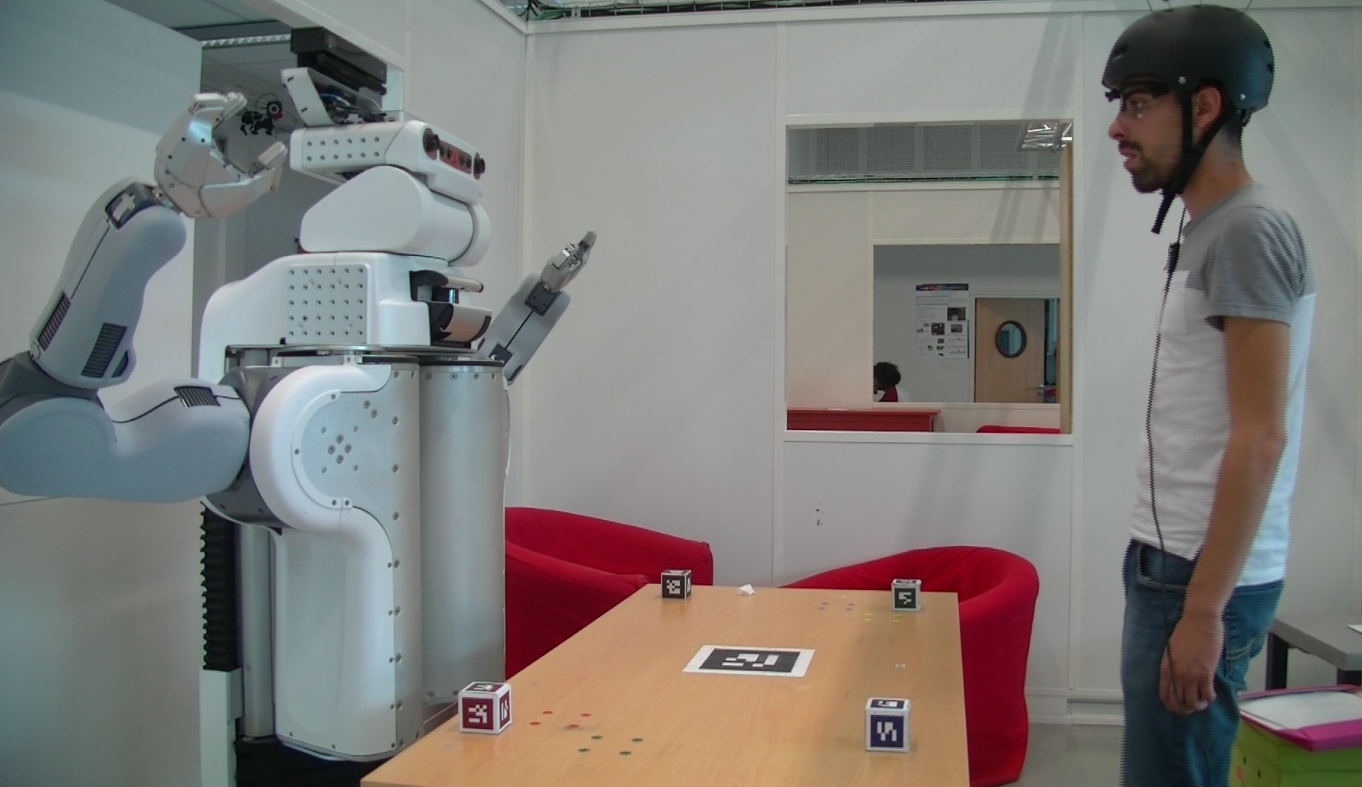
\includegraphics[width=0.45\textwidth]{figs/Chapter6/VideoInit.png}
       \label{subfig:videoInit}
   }
    %~
	\subfigure[End of the interaction. The stack should follow a precise order (red, black, blue, green).]{
        \centering
        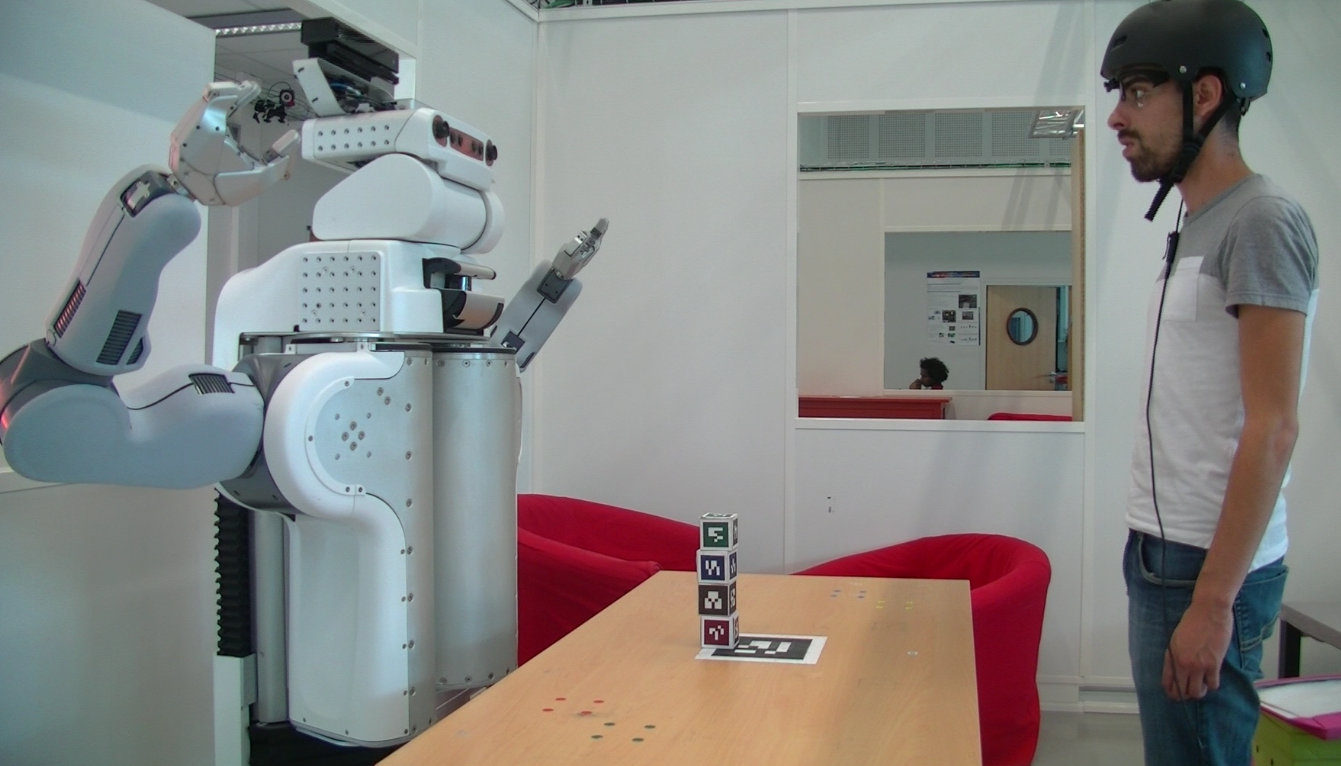
\includegraphics[width=0.45\textwidth]{figs/Chapter6/VideoGoal.png}
       \label{subfig:videoGoal}
   }
    \caption{Task used in the on-line video based study. In this task a human and a robot have to build a stack of colored cubes. Different head behaviors of the robot was compared in the videos.}
    \label{fig:videoTask}
\end{figure*}

\subsection{Anticipation of robot actions}

The first behavior we studied concerns when the robot is performing actions. We asked ourselves if the fact that the robot anticipates its next action with its head would benefit to the Joint Action and more particularly to the understanding of the robot actions by the human. To do so, we asked people to watch two videos: one with anticipation and one without. These two videos are focused on the first part of the interaction where the robot put the first two cubes on the stack. In the video without anticipation, the robot simply looks at the cube it is picking and the support where it is placing the cubes (as described in the "basic behavior"). In the video with anticipation the robot still looks at the cube it is picking and the supports where it is placing the cubes. However the robot starts looking at the second cube to put on the stack while it is retracting from its first action (putting the first cube).

After having watched the two videos, participants were asked to answer several questions for each video. There was 4 5-scales questions for each video concerning the predictability of the robot behavior and the fact that the robot head behavior was adequate, clear and useful to the interaction. Then, the participants were asked to choose which video they preferred between the two videos (with the possibility to select both). These questions can be found in Appendix~\ref{chap:annexe2}. We also let a free space for comments at the end of the questionnaire.

The results of the questionnaire for this scenario can be found in Fig.~\ref{fig:resSce1}. No significant difference was found between the conditions either concerning the scores in the 5-scales questions (p=0.3467) or the preferences (p=0.3711). Indeed, based on the free comments of the participants, we found that they had difficulties to find the differences between both conditions, and, when they found the differences, they were sometime disturbed by the fact that the robot looks at an object without acting (in the condition with anticipation). 

We can conclude that the way we implemented anticipation is not conclusive for Joint Action, or at least for the kind of task tested here. Indeed, one factor here is that the task and needed actions are well known of both participants (as the stack order is predetermined, there is only one action to do at each time). Consequently, the anticipation may not be needed here but may be more interesting in a scenario where the human does not know the next robot action. Moreover, maybe the way the anticipation behavior is implemented is not the best way to do it. Further investigations may be needed on this subject.

\begin{figure*}[!h]
\centering
	\subfigure[Scores on the questions asked for each video of the scenario concerning the anticipation of robot actions. The score is the addition of the rates (in a scale of 5) of the 4 questions.]{
        \centering
        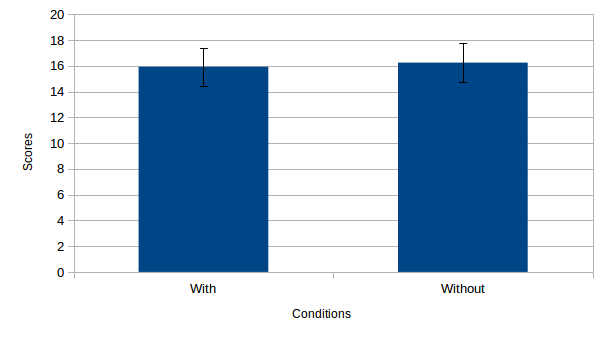
\includegraphics[width=0.45\textwidth]{figs/Chapter6/ScoresSce1.png}
       \label{subfig:scoresSce1}
   }
    %~
	\subfigure[Preferences for the scenario concerning the anticipation of robot actions. Numbers represent the number of times where a video was chosen for the preference question (on 59 participants).]{
        \centering
        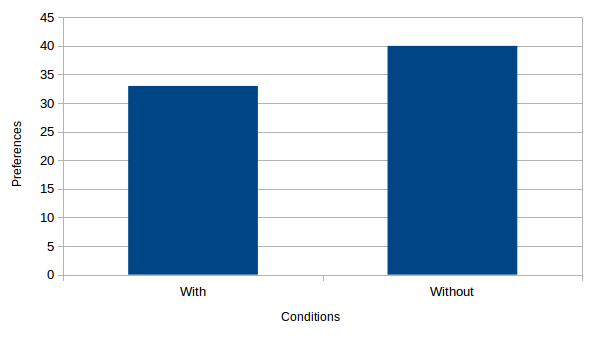
\includegraphics[width=0.45\textwidth]{figs/Chapter6/PrefSce1.png}
       \label{subfig:prefSce1}
   }
    \caption{Results for the scenario concerning the anticipation of robot actions. No significant differences was found between the two conditions (with anticipation and without anticipation).}
    \label{fig:resSce1}
\end{figure*}



\subsection{Following human's activity}

We then studied how the robot should show that it follows and understands human's actions. We want here to find a behavior adapted to the information the robot has concerning the human. In our system, the robot detects the human with a motion capture system (see description in Introduction) and has information about the head and the right hand positions and orientations. Here we tried to find a relatively simple behavior which, with a minimum of information allows the robot to show its attention and understanding. First, we compared different ways to decide when to look at the human's hand or when to look at the human's head. We compared three different conditions with videos based on the end of interaction (the part where the human puts the two last cubes). In all videos the human puts the two cubes one after the other. He also records a stop time during his first action by hesitating a short moment. In one condition, the robot looks at the human's hand whenever the hand is moving and looks at the human's head when the hand is not moving (with a small hysteresis in order to avoid going back and forth between the hand and the head). In the second condition, the robot looks at the human's hand whenever the hand is into a "working area" and at the human's head whenever the hand is not in the area. This "working area" is basically all the volume above the table. In the last condition, the robot looks at the human's hand whenever the hand is in the "working area" and is moving. Else the robot looks at the human head.

In the same way as for the previous scenario, participants were asked to answer several questions for each video. There was 4 5-scales questions for each video concerning the understanding of the human's actions by the robot and the fact that the robot head behavior was adequate, clear and useful to the interaction. Then, the participants were asked to choose which video they preferred between the three videos (with the possibility to select several). These questions can be found in Appendix~\ref{chap:annexe2}. We also let a free space for comments at the end of the questionnaire.

\begin{figure*}[!h]
\centering
	\subfigure[Scores on the questions asked for each video of the first scenario concerning the following of human's activity. The score is the addition of the rates (in a scale of 5) of the 4 questions.]{
        \centering
        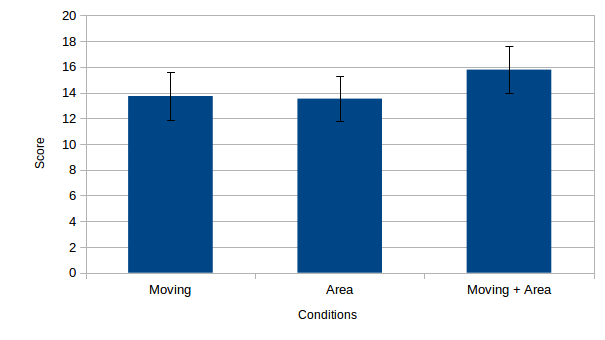
\includegraphics[width=0.45\textwidth]{figs/Chapter6/ScoresSce2.png}
       \label{subfig:scoresSce2}
   }
    %~
	\subfigure[Preferences for the first scenario concerning the following of human's activity. Numbers represent the number of times where a video was chosen for the preference question (on 59 participants).]{
        \centering
        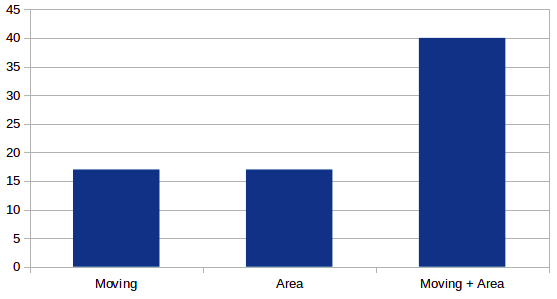
\includegraphics[width=0.45\textwidth]{figs/Chapter6/PrefSce2.png}
       \label{subfig:prefSce2}
   }
    \caption{Results for the the first scenario on the following of human's activity. The conditions where the robot looks at the human's hand whenever it is in a "working area " and moving has been significantly preferred to the two others.}
    \label{fig:resSce2}
\end{figure*}

The results of the questionnaire for this scenario can be found in Fig.~\ref{fig:resSce2}. The third condition (where the robot is considering area and movement) has been evaluated significantly higher than the two others (p < 0.01). No significant difference has been found between the two others videos. These results gives us leads for the construction of a robot head behavior. Indeed, we can see that with a minimal robot behavior (a simple switch between the hand and the head based on the hand position and movement), the robot is able to show its attention and understanding in a relatively acceptable way (rated at 15.78/20 in the 5-scale questions by the participant).

Then, we asked ourselves if, when an action of the human is detected by the robot, the robot should show its understanding of the action by recording a small stop on the action. We asked participant to watch two videos. These videos were also based on the end of interaction (the part where the human puts the two last cubes). In each video the human puts the two cubes one after the other and the robot was looking at human's hand and head following the third behavior described previously (where the robot considers area and movement). Additionally, in one video, the robot was making a stop on the stack each time the human placed a cube on it. The participants were asked to answer the same questions as for the previous scenario.

\begin{figure*}[!h]
\centering
	\subfigure[Scores on the questions asked for each video of the second scenario concerning the following of human's activity. The score is the addition of the rates (in a scale of 5) of the 4 questions.]{
        \centering
        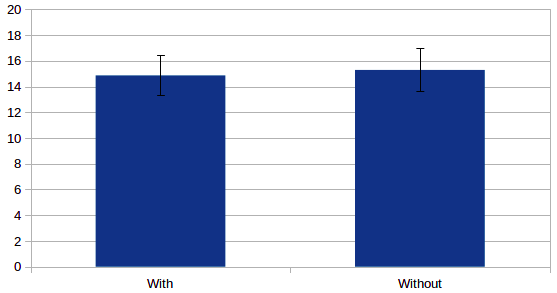
\includegraphics[width=0.45\textwidth]{figs/Chapter6/ScoresSce3.png}
       \label{subfig:scoresSce3}
   }
    %~
	\subfigure[Preferences for the second scenario concerning the following of human's activity. Numbers represent the number of times where a video was chosen for the preference question (on 59 participants).]{
        \centering
        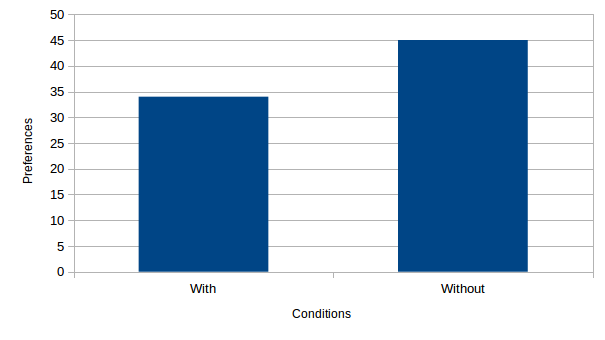
\includegraphics[width=0.45\textwidth]{figs/Chapter6/PrefSce3.png}
       \label{subfig:prefSce3}
   }
    \caption{Results for the second scenario on the following of human's activity. One condition includes a stop after each action of the human (With) while the other corresponds the the third behavior of the previous scenario (Without).}
    \label{fig:resSce3}
\end{figure*}

The results of the questionnaire for this scenario can be found in Fig.~\ref{fig:resSce3}. No significant difference was found between the conditions either concerning the scores in the 5-scales questions (p=0.33) or the preferences (p=0.1093). Indeed, based on the free comments of the participants, we found that they had difficulties to find the differences between both conditions, and, when they found the differences, they sometime disliked the fact that, when the robot makes a stop (in the condition with as stop), the robot does not follow anymore what the human is doing.


\subsection{Signaling human's actions}

Then, we bear interest to the signals the robot should give with its head concerning the Shared Plan execution. In this part, the videos were based on the middle of the interaction (the second cube of the robot and the first of the human).

The first signal we identified as potentially interesting concerns the signaling of an action the human should perform and is not performing. In all tested videos, the robot was putting its second cube on the stack, then, the human was waiting a few moment before putting his cube. In one video, the robot was not giving any signal to the human, it was just following the "basic behavior" described earlier. In the two others videos, after a small waiting time, the robot gave a signal to the human for him to place his cube on the stack. In one video, the signal consisted on looking at the cube to take and then looking back at the human's head. In the other video, the signal consisted on looking at the cube, then looking at the stack and finally looking back at the human's head.

In the same way as for the previous scenarios, participants were asked to answer several questions for each video. There was 3 5-scales questions for each video which concerned the fact that the robot head behavior was adequate, clear and useful to the interaction. Then, the participants were asked to choose which video they preferred between the three videos (with the possibility to select several). These questions can be found in Appendix~\ref{chap:annexe2}. We also let a free space for comments at the end of the questionnaire.

\begin{figure*}[!h]
\centering
	\subfigure[Scores on the questions asked for each video of the first scenario concerning the signaling of human's actions. The score is the addition of the rates (in a scale of 5) of the 3 questions.]{
        \centering
        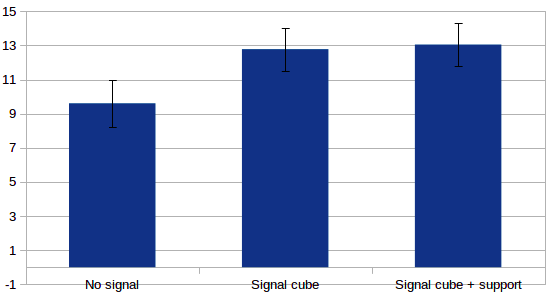
\includegraphics[width=0.45\textwidth]{figs/Chapter6/ScoresSce4.png}
       \label{subfig:scoresSce4}
   }
    %~
	\subfigure[Preferences for the first scenario concerning the signaling of human's actions. Numbers represent the number of times where a video was chosen for the preference question (on 59 participants).]{
        \centering
        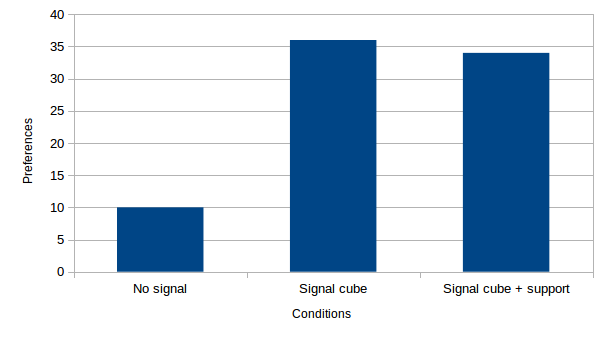
\includegraphics[width=0.45\textwidth]{figs/Chapter6/PrefSce4.png}
       \label{subfig:prefSce4}
   }
    \caption{Results for the first scenario on the signaling of human's actions. In one condition the robot was not giving any signal to the human (No signal). In another conditions the robot was giving a signal consisting of looking at the cube to place and looking back at the human's head (Signal cube). In the last condition the robot was giving a signal consisting of looking at the cube to place, the stack and then looking back at the human's head (Signal cube + stack).}
    \label{fig:resSce4}
\end{figure*}

The results of the questionnaire for this scenario can be found in Fig.~\ref{fig:resSce4}. The first condition (where there is no signal) has been evaluated significantly lower than the two others (p < 0.01). No significant difference has been found between the two different signals given by the robot. These results show us that the studied signal (the robot signals to the human that he should act when he is not acting) is considered important by peoples. One possible explanation concerning the lack of difference between the two ways tested to perform the signal is that, in this task, there is only one place where to put the cube. Indeed, in the signal where the robot looks at the stack, the information given is not so interesting in this configuration. Further investigations can be interesting with scenarios where the human has several choices of actions to execute.

Then, we investigated the use of a signal to help turn-taking. We specifically focused on the signal needed at the end of a robot action if the next action to be performed is a human action. In this scenario, we compared 4 videos where the robot puts its second cube and then the human puts his first cube. In two videos the robot was giving a signal to the human at the end of its action. This signal consisted in looking at the human's head, looking at the cube he should put on the stack and then looking back at the human's head. In one of these two videos, the robot was giving the signal while retracting from its action. In the other the robot was giving the signal after retracting from its action. In the two other videos, the robot was not giving signal to the human. In one case its looks at the human's head as soon as its action is over(while retracting), in the other case it looks at the human's head only after retracting from its action. The participants were asked to answer the same questions as for the previous scenario.

\begin{figure*}[!h]
\centering
	\subfigure[Scores on the questions asked for each video of the second scenario concerning the signaling of human's actions. The score is the addition of the rates (in a scale of 5) of the 3 questions.]{
        \centering
        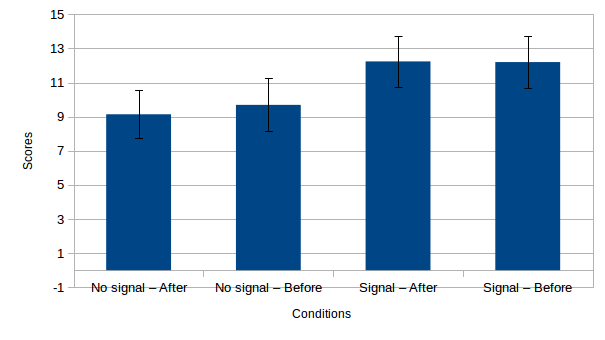
\includegraphics[width=0.45\textwidth]{figs/Chapter6/ScoresSce5.png}
       \label{subfig:scoresSce5}
   }
    %~
	\subfigure[Preferences for the second scenario concerning the signaling of human's actions. Numbers represent the number of times where a video was chosen for the preference question (on 59 participants).]{
        \centering
        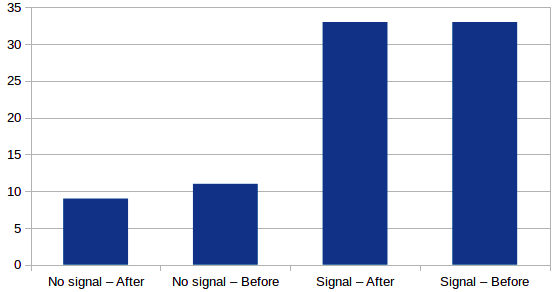
\includegraphics[width=0.45\textwidth]{figs/Chapter6/PrefSce5.png}
       \label{subfig:prefSce5}
   }
    \caption{Results for the second scenario on the signaling of human's actions. In one condition the robot was not giving any signal to the human and was looking at his head after retracting (No signal - After). In another condition, the robot was not giving any signal to the human and was looking at his head while retracting (No signal - Before). In the two others conditions the robot was giving a signal consisting in looking at the the human's head, looking at the cube to place on the stack and looking back at the human's head. In one condition the robot was giving the signal after retracting from its action (Signal - After) and in the other while retracting (Signal - Before).}
    \label{fig:resSce5}
\end{figure*}

The results of the questionnaire for this scenario can be found in Fig.~\ref{fig:resSce5}. The two conditions where there is a signal have been evaluated significantly higher than the two others (p < 0.01). No significant difference has been found between the two conditions with a signal as well as for the two conditions without a signal. These results show the usefulness of a signal at the end of robot actions in order to help turn-taking. However, apparently the timing of the signal (during or after retracting) has not been found important by the users. 

\subsection{Finding the priority target}

In the last scenario of the study, we focused on the decision to take when the robot has several possible target to look at. We studied here the case where the robot is executing an action (and so has a target for its action) and the human performs another action at the same time (and so the robot should also look at the human's action). In the videos, the robot is still placing its second cube on the stack when the human picks his next cube (in prevision of placing it on the stack). In each video, the robot looks at the stack when putting its cube. In one video, the robot does not look at all at the human action. In another video, the robot looks at the human action (it looks at the human's hand and goes back to the stack) when it is executed without interrupting its action. In the last video, the robot stops its action to look at the human action and then restarts its action.

In the same way as for the previous scenarios, participants were asked to answer several questions for each video. There was 3 5-scales questions for each video concerning the fact that the robot behavior was adequate, clear and useful to the interaction. Then, the participants were asked to choose which video they preferred between the three videos (with the possibility to select several). These questions can be found in Appendix~\ref{chap:annexe2}. We also let a free space for comments at the end of the questionnaire.

\begin{figure*}[!h]
\centering
	\subfigure[Scores on the questions asked for each video of the scenario concerning the priority target. The score is the addition of the rates (in a scale of 5) of the 3 questions.]{
        \centering
        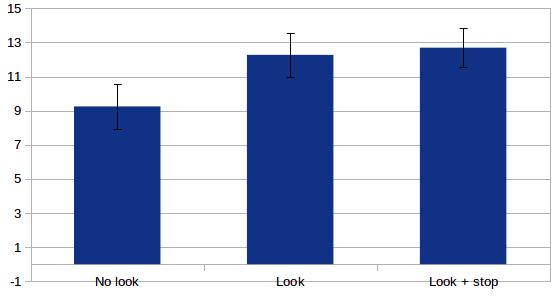
\includegraphics[width=0.45\textwidth]{figs/Chapter6/ScoresSce6.png}
       \label{subfig:scoresSce6}
   }
    %~
	\subfigure[Preferences for the scenario concerning the priority target. Numbers represent the number of times where a video was chosen for the preference question (on 59 participants).]{
        \centering
        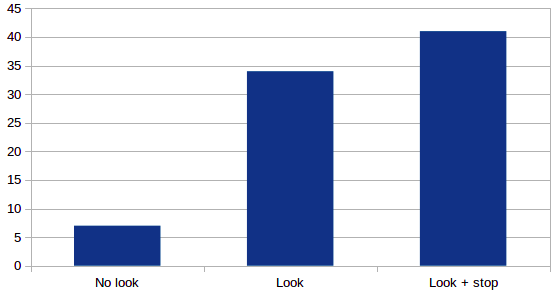
\includegraphics[width=0.45\textwidth]{figs/Chapter6/PrefSce6.png}
       \label{subfig:prefSce6}
   }
    \caption{Results for the scenario concerning the priority target. In one condition the robot was not looking at the human's action (No look). In another condition the robot was looking at the human's action without interrupting its action (Look). In the last condition the robot was interrupting its action to look at the human's action (Look + stop).}
    \label{fig:resSce6}
\end{figure*}

The results of the questionnaire for this scenario can be found in Fig.~\ref{fig:resSce6}. The condition where the robot does not look at the human's action has been evaluated significantly lower than the two others (p < 0.01). No significant difference has been found between the two conditions where the robot looks at the human's action. These results show us that even if the robot is busy doing something else it is important that it looks at human's action to acknowledge the fact that it perceived the action. If the robot action requires the full focus of the robot head, the robot can interrupt briefly its action in order to look at the human's action without degrading the acceptability of its behavior.


\section{The robot head behavior}

Based on our previous analysis and the performed on-line user study we start conceiving an architecture to generate a robot head behavior. This behavior is for now computed based on a Joint Action with only one human.

The architecture can be found in Fig.~\ref{fig:headArchi}. We can find in this architecture the four "families" described in Sec.~\ref{sec:reflection} (human observation, robot action, dialogue and coordination). Based on informations concerning humans, the robot constantly computes a target (either an object or a part of the human body) to look at. In addition, when the robot is performing an action, it also computes a target for the action. In a same way, when the robot is conversing with a human, another target is computed. Based on the current state of the Shared Plan, the robot also computes signals to give to the human. Finally, based on the different targets and signals, an arbitration module chooses at each time the final target to look.

\begin{figure}[!h]
	\centering
    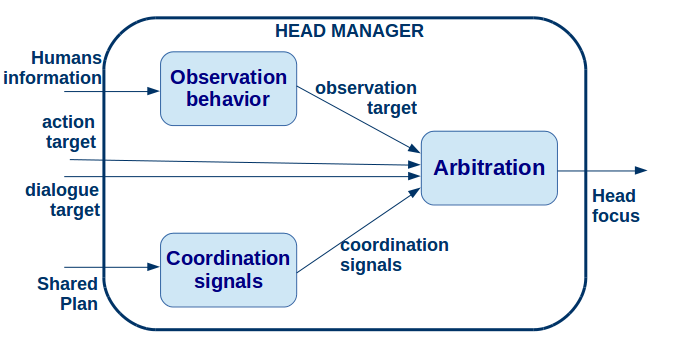
\includegraphics[width=0.9\textwidth]{figs/Chapter6/Head_archi.png}
    \caption{The architecture to generate the robot head behavior. The arbitration modules chooses where the robot should look based on several possible behaviors and signals. The possible behaviors concern the human activity, the current robot action and the current state of the dialogue. Coordination signals are computed based on the current Shared Plan.}
    \label{fig:headArchi}
\end{figure}

In this architecture, a target is described as a point to look at (either an object or a part of the human body) and an associated priority.
$$target = <point, priority>$$
A signal is described as an ordered set of points to look at with associated durations, a priority, an expiration time and possibles expiration conditions (events).
$$signal = <points, durations, priority, expiration_time, expiration_conditions>$$

This architecture is still a work in progress, there are still needs of deepening for some parts and the parametrization of the priorities and durations are still needed.

\subsection{Observation target}

We saw previously that the robot should show its interest and understanding of the human activity. We studied in the previous section how we can show the interest of the robot in the human's actions based on the position and movements of his hand. We keep the condition of the study which was the most highly marked: the robot looks at the human's hand whenever the hand is moving (with a small hysteresis in order to avoid going back and forth between the hand and the head) and into a "working area". Working areas can be defined dynamically and attached to objects (e.g. everything above a table).

Additionally to this behavior, another important feature is joint attention. When the human stares at an object for a sufficient time, the robot should also look at this object. In a same way, if the human stares at the robot, the robot should return his look. The given algorithm to compute the point corresponding to the human observation can be found in Alg.~\ref{alg:observation}.


\begin{algorithm}
\caption{Computation of the point to look based on human's activity}
\label{alg:observation}
\begin{algorithmic}
\REQUIRE human's hand position and movement, objects position, human's  head position and target
\IF {human's head target = robot > t}
\STATE $point = human's \ head$\hfill \textit{$\vartriangleright$ the human stares at the robot}
\ELSIF{human's head target = object > t}
\STATE $point = object$\hfill \textit{$\vartriangleright$ the human stares at an object}
\ELSIF{human's hand is moving $\&$ human's hand is in "working area"}
\STATE $point = human's \ hand$\hfill \textit{$\vartriangleright$ following human's action}
\ELSE
\STATE $point = human's \ head$\hfill \textit{$\vartriangleright$ by default, looking at human's head}
\ENDIF
\RETURN $point$
\end{algorithmic}
\end{algorithm}

This behavior is for now really basic. One the reason is that we want a behavior which can work with few information concerning the human (here only concerning the head and one hand). Moreover, we strongly think, even if it remains to be proved, that a minimal behavior is sometime preferred to a more complex one as soon as all the needed components are here.

\subsection{Robot action and dialogue targets}

We saw the importance of having a head behavior in adequacy with the robot current action. Consequently, the action target is computed directly by the component in charge of executing robot actions and depends of the action executed. The point to look at is in most cases the "target" object (e.g. the object to pick or the support where to place). The priority associated with this point principally depends of the fact that the action requires the head focus (e.g. at the beginning of a pick action, the priority will be higher to ensure the good perception of the object). The module in charge of executing actions has also access to the point the robot is looking at in order to adapt the action execution (e.g suspend if necessary).

In a same way, the target associated to dialogue is directly computed by the module in charge of the dialogue. It mainly consists in looking at the human when talking and at the objects the robot is referring to.

\subsection{Coordination signals}

We saw the importance of coordination signals during Joint Action execution. In this work, these signals are based on the execution of the Shared Plan. The first two signals are the one studied in the on-line study. The first one is computed whenever a human has an action to execute and is not performing it after a certain amount of time (and that he is not doing another action). In this case, the robot signals to the human the action he should execute. This signal consist of looking at the human's head, then the different points of interest of the action to execute and finally looking at the human's head again. The points of interest of an action are ordered and defined for each high level action (e.g. for the pick and place action it is the object to pick and, then, the support where to place). This signal should have a relatively long expiration  time as its timing is not crucial. It should also have the execution of the awaited action in its expiration conditions.

Another signal concerns the help of turn-taking. After each robot action, if this action unlocks another action attributed to the human (there is a causal link between the two actions), the robot sends a signal to the human to execute the action. This signal consists of looking at the human's head, then the different points of interest of the action to execute and finally looking at the human's head again. This signal should have a small expiration time as it has to be performed just after the robot action. It should also have the execution of the awaited action in its expiration conditions.

Finally, we saw the importance of looking at a human's actions, even if the robot is currently busy doing something else. To do so, when the human performs an action, a signal is computed with a high priority as well as a small expiration time because the signal does not make sense if it comes latter after the action. This signal consists of looking a the point of interest of the executed action. 

\subsection{Arbitration}

The arbitration of the different points to look at and the different signals to send is based on priorities. The arbitration module first chooses the point to look at with the higher priority between the ones from human observation, dialogue and robot action. Then, when a signal is sent by the coordination module, it is stored in a waiting list (ordered by priorities). If the priority of a signal in the waiting list is higher than the current priority, the robot executes the signal. In order to keep signals consistent, a signal started can not be interrupted even if there is another signal or point to look at with a higher priority. When a signal expires (the expiration time is reached or an expiration condition is true) the signal is removed from the waiting list.

There may be some missing signals in the current version of the architecture. However, we strongly think that it has been done in a sufficiency generic way in order to integrate new signals if needed.

\section{Conclusion}

In this chapter, we studied non-verbal behavior during human-robot Joint Action, and more especially the robot head behavior. A first bibliographic study has been done in order to identify the needed components of a robot head behavior adapted to the Joint Action. Then, some specific parts of these components have been studied with an on-line video based study. Finally, an architecture to generate the robot head behavior has been proposed. This architecture, still in construction, should allow the robot to produce a head behavior which provides the needed information in order for the robot to show its attention, make its action understandable, dialogue and coordinate the  Joint Activity based on the Shared Plan.

\ifdefined\included
\else
\bibliographystyle{StyleThese}
\bibliography{These}
\end{document}
\fi
